% !TEX encoding = UTF-8 Unicode

\documentclass[a4paper]{article}

\usepackage{color}
\usepackage{url}
\usepackage[T2A]{fontenc} % enable Cyrillic fonts
\usepackage[utf8]{inputenc} % make weird characters work
\usepackage{graphicx}
\usepackage{booktabs}
\usepackage{adjustbox}

\usepackage[english,serbian]{babel}
%\usepackage[english,serbianc]{babel} %ukljuciti babel sa ovim opcijama, umesto gornjim, ukoliko se koristi cirilica

\usepackage[unicode]{hyperref}
\hypersetup{colorlinks,citecolor=green,filecolor=green,linkcolor=blue,urlcolor=blue}

%\newtheorem{primer}{Пример}[section] %ćirilični primer
\newtheorem{primer}{Primer}[section]

\begin{document}

\title{Kvantna kriptografija\\ \small{Seminarski rad u okviru kursa\\Tehničko i naučno pisanje\\ Matematički fakultet}}

\author{Igor Glišović\\mi22292@alas.matf.bg.ac.rs\\\\ Željko Zekavičić\\mi22130@alas.matf.bg.ac.rs\\\\ Nađa Lazarević\\mi22175@alas.matf.bg.ac.rs\\\\ Ana Mladenović\\mi22119@alas.matf.bg.ac.rs\\\\}
\date{18.~decembar 2022.}
\maketitle

\abstract{
Čuvanje podataka sa klasičnom kriptografijom u moderno doba postaje teže, jer su se sa razvojom tehnologija razvijali i načini za lakše saznavanje tajnih ključeva. Javila se velika potreba za načinom na koji se može spoznati da li sistemu pristupaju treća lica. Rešenje se može naći primenom principa kvantnih čestica u sistemu kvantne mehanike i njihove neodređenosti i sprezanja na zaštitu informacionih sistema.

\tableofcontents

\newpage

\section{Uvod}
\label{sec:uvod}
Kriptografija je nauka koja se bavi očuvanjem tajnosti informacija. Cilj je da se informacije prenesu od pošiljaoca do primaoca tako da smo sigurni da one nisu dospele do nekog trećeg lica. Pri samom nastanku kriptografije glavni problemi su bili na koji način sačuvati tajnost procesa enkripcije/dekripcije podataka (neki od prvih primera klasične kriptografije su Cezarova šifra\footnote{Cezarova šifra (1. vek p.n.e) se zasnivala na supstituciji, gde bi se pri šifriranju svaki karakter pomerio unapred za n-pozicija u alfabetu, a pri dešifrovanju pomerio unazad za n-pozicija}  i Skital\footnote{Skital (5. vek p.n.e) je parče štafete koji su Grci koristili kako bi obavijali sakrivenu poruku oko nje i nakon toga došli do ispravne poruke}), jer bi se nakon saznavanja procesa na koji se šifruju podaci, oni mogli lako dešifrovati.

Nakon mnogo vekova, nastankom i razvojem informacionih tehnologija, očuvanje sigurnosti podataka postaje još bitnije (ali i teže) nego što je nekad bilo. Kao jedan od najboljih načina za enkripciju podataka iz ere klasične kriptografije izdvaja se Vernamova šifra\cite{mariokvantna} tzv. \textit{OneTimePad} - OTP). OTP se zasniva na principu generisanja nasumičnog dugačkog ključa dužine kao izvorna poruka koju šaljemo. Ovakav sistem radi samo ako svaki put generišemo novi kod, jer ako dva puta prosledimo isti, lako se može dešifrovati ono što smo poslali. Takođe, veliki problem kod ovakvog načina enkripcije predstavlja prenos dugačkog ključa, te bi sam proces slanja poruke trajao duže. Ovaj problem se rešava tako što ključ skraćuje na fiksnu dužinu za svaku poruku. Međutim, moderna kriptografija sada nailazi na novi problem (poznatiji kao Kvaka 22):

 \begin{center}
\textit{Komunikacija između pošiljaoca i primaoca je sigurna, samo ako znamo da je sigurna.}
\end{center} 

Ovde dolazimo do zaključka da se klasičnom kriptografijom nikako ne može znati da li je informacija kompromitovana od strane trećih lica u toku slanja poruke. Ovaj problem se rešava primenom osobina kvantne mehanike na prenos informacija u nekom informacionom sistemu.
\section{Istorijat}	
\label{sec:istorijat}

Kroz celu istoriju čovečanstva postojala je potreba za sigurnom razmenom informacija. Problemom sigurne komunikacije bavili su se već Egipćani i Indijci pre više od 3000 godina i od tada do danas osnovna ideja se nije promenila, preneti neku poruku s jednog mesta na drugo što je sigurnije moguće.

Krajem dvadesetog veka čovečanstvo je ušlo u eru informacionih tehnologija. IT industrija, koja se bavi proizvodnjom, obradom, skladištenjem i prenosom informacija, postala je sastavni deo globalnog ekonomskog sistema, potpuno nezavisan i prilično značajan sektor privrede. Zavisnost savremenog društva od informacionih tehnologija je toliko velika da propusti u informacionim sistemima mogu dovesti do značajnih incidenata. Telekomunikacije su ključna industrija informacionih tehnologija. Međutim, informacije su tokom transporta veoma osetljive na razne vrste zloupotreba. Jedinice za skladištenje i obradu podataka mogu biti fizički zaštićene od nedobronamernih, što se ne može reći za komunikacione linije koje se protežu na stotine ili hiljade kilometara i koje je gotovo nemoguće zaštititi. Stoga je problem zaštite informacija u sferi telekomunikacija veoma značajan. Kriptologija kao nauka i posebno njen deo kriptografija upravo se bave ovom problematikom.

Dugi niz godina su mnogi naučnici tražili način ostvarenja takve komunikacije između dve osobe koja bi garantovala privatnost. Kvantna kriptografija je relativno novija oblast koja se bavi obezbeđenjem sigurne komunikacije između pošiljaoca i primaoca informacije, koristeći zakone kvantne fizike. Cilj rada je da se upoznamo sa principima kvantne distribucije ključa (o čemu će biti reči u sekciji \ref{qkd}) za kodiranje informacija i osnovnim problemima koji se javljaju pri njegovoj realizaciji.

Kvantna kriptografija je prvi put predstavljena\cite{draganakvantna} od strane Stephena Weisnera, na Kolumbija Univerzitetu u Njujorku, koji je ranih 70-ih godina prošlog veka predstavio koncept kvantnog kodiranja. Njegov rad, pod naslovom,,Kodiranje konjugata" (engl. Conjugate Coding) je bio odbačen od strane žurnala IEEE Informaciona Teorija, ali ipak biva objavljen 1983. godine u SIGACT News. U tom radu on je pokazao kako smestiti i poslati dve poruke koje su kodirane u dve srodne pojave", kao što je linearna i cirkularna polarizacija svetla, tako da bilo koja, ali ne obe, mogu biti po- slate, primljene i dekodirane. Svoju ideju je ilustrovao kroz novčanice koje je nemoguće falsifikovati. U međuvremenu, Charles H. Bennet\cite{sandrakvantna} (koji je znao o Weisnerovoj ideji) i Gilles Brassard su počeli raditi na istom području, najpre kroz nekoliko članaka, a posle i eksperimentalnim prototipom koji je demonstrirao tehnološku ostvarivost koncepta. Taj se prototip sastojao od fotona koji su se provlačili kroz 0.30 m dugu cev. Smer u kojem su fotoni oscirali te njihova polarizacija predstavljaju 0 ili 1 niza kvantnih bitova ili kubita. Nezavisno od njih Artur Ekert sa univerziteta u Oksfordu je 1990. godine razvio drugačiji pristup kvantnoj kriptografiji zasnovanoj na kvantnim korelacijama poznatim kao kvantna isprepletanost.
\section{Principi kvantne kriptografije}
Kvantna mehanika\cite{stevankvantna} se zasniva na sledećim aspektima:
\begin{itemize}
\item aspekt prirodne neodređenosti, isprepletanosti - superpozicije, odnosno da se čestice koje postoje ne nalaze samo na jednom mestu (mogu se naći na dva mesta istovremeno)
\item aspekt kvantnog sprezanja, što znači da su dve nezavisne čestice uvek nerazdvojno povezane, čak iako ne postoji mogućnost njihovog međusobnog delovanja
\item delovanje jedne čestice na drugu, pa čak i odmeravanje, promeniće prirodu druge čestice
\end{itemize}
Ovi aspekti su ključni za kvantnu kriptografiju, jer obezbeđuju sigurnost očuvanja ključa.
\subsection{Kvantni računari}
Ključna razlika između klasičnih računara i kvantnih računara je vid predstavljanja podataka. Na klasičnim račuanrima, podaci se predstavljaju pomoću bitova (0,1), dok se na kvantnim predstavljaju u kvantnim bitovima - kubitima. Kubit može biti neka mikro ili nano čestica (foton, elektron, atom) i radi uz pomoć nekog mikrokontrolera koji će joj zadati sledeće stanje (smer rotacije). Sve informacije se kodiraju u tzv. kvantna (neortogonalna) stanja. U našem slučaju podatke prenosimo putem optičkih kablova, a osnovne čestice su fotoni. Fotoni se pri kretanju rotiraju pod nekim uglom, a kada se više fotona rotira u istom smeru, onda su oni polarizovani fotoni. Polarizacioni filteri propištaju isključivo fotone koji su polarizovani u jednom određenom smeru, a ostale blokiraju. Prepoznavanje promene smera je zapravo indikacija da neko pokušava da sazna informacije, jer je pokušao da sazna ključ, a samim tim promenio smer rotacije nekih kubita.


Potencijal kvantnih računara je veliki jer bi se za n-operacija kod klasičnog računara, sa istim brojem kubita kod kvantnog računara moglo uraditi $ 2^{n} $ operacija (eksponencijalno rastući kapacitet). 
\subsection{Kvantni protokoli}
\label{qkd}
Kvantni protokoli\cite{stjepankvantna} postoji zato što postoji razlika u distribuciji kvantnih ključeva (engl. QKD - Quantum Key Distribution), te razlikujemo nekoliko različitih protokola:
\begin{itemize}
\item BB84 protokol - prvi i najrasprostranjeniji protokol. Koristi jedan jednosmerni kvantni kanal i jedan dvosmerni javni kanal; bazira se na 4 neortogonalna stanja koja se mogu videti na Slici \ref{slike:prva}. 
\item B92 protokol - koristi 2 neortogonalna stanja.
\item E91 protokol (Ekertova šema) - koristi isprepletani par fotona.
\item SARG04 - otporniji BB84.
\item Protokol šest stanja  - tri para ortogonalnih polarizacionih stanja (najnoviji, ali najmanje efikasan).
\end{itemize}
\begin{figure}[h]
\centering
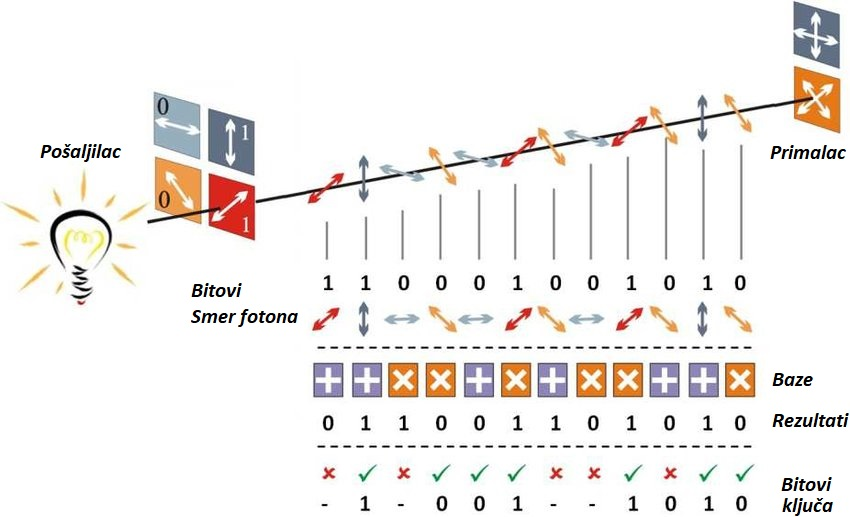
\includegraphics[width=0.8\textwidth]{bb84.jpg}

\caption{Metodika rada BB84 protokola}
\label{slike:prva}
\end{figure}
\subsection{Kvantna razmena ključa}
Sigurni prenos informacija nemoguće je izvesti bez sigurnog prenosa ključa, stoga postoji nekoliko setova pravila (protokola) koje koristimo pri razmeni ključeva, a mi ćemo navesti dva najosnovnija.\newpage
Prvi tip je \emph{"pripremi i izmeri"} tip protokola. On se zasniva na aspektu neodređenosti kvantnih čestica. Ovaj protokol koristi svojstvo kjubita da promene stanje u odnosu na drugu česticu i tako otkriva potencijalan napad trećeg lica na ključ.

Drugi tip je zasnovan na osobini isprepletanosti kubita. Kubiti se kombinuju u veće celine (blokove kubita). Protokol kontroliše da se moguće greške u prenosu kao što je šum, ne poistoveti sa neovlašćenim napadom.
\smallskip
\subsection{Vrste napada na sisteme i odbrana}
Postoji nekoliko vrsta napada na kvantne kriptografske sisteme, i to:
\begin{itemize}
\item "Middleman" (središnja osoba) napad - dešava se jer nismo obezbedili autentifikaciju u sistemu
\item PNS (photon-number splitting) napad - koriste oslabljene laserske pulseve kako bi došli do male količine informacije
\item Hakerski napadi - ciljaju nesavršenost u implementacijama
protokola umesto samih protokola (najčešće koriste lažna stanja ili "Trojance")
\item DOS (Denial of Service) napad - blokiranje protoka informacije, "presretanje"
\end{itemize}
Kvantni kriptografski sistem biće siguran ako i samo ako obezbedimo da će svi delovi sistema raditi besprekorno. Moramo da se postaramo da nijedno treće lice ne može da pristupi uređajima za enkripciju/dekripciju koji se nalaze kod pošaljioca/primaoca informacije koje prenosimo. Pored toga moramo obezbediti da se svaki put generiše potpuno nasumična vrednost ključa (bez ikakve mogućnosti nalaska pravilnosti).  Na kraju, moramo obezbediti da naš komunikacioni medijum ima siguran proces autentifikacije (potvrda identiteta).

\section{Implementacija kvantne kriptografije}
Naučnici su pokazali da kvantna distribucija ključa funkcioniše, ali se ne koristi previše zbog značajnih tehnoloških ograničenja. Da bi poslao kvantni ključ, laser sa jednim fotonom emituje signal, preko optičkog kabla. Ova metoda je sporija od trenutnih telekomunikacionih tehnologija i zahteva namenski optički kabl između dve strane. Na primer, multinacionalna kompanija Amazon nije mogla da obezbedi transakcije klijenata korišćenjem kvantne enkripcije, jer bi joj bili potrebni kablovi između njenih internih servera i pojedinačnih uređaja koji vrše kupovinu. Udaljenost je takođe faktor. Kada se optički kablovi koriste za prenos podataka, kao u vašem kućnom internetu i kablovskim sistemima, oni koriste repetitore za slanje podataka na veće udaljenosti. Međutim, ti repetitori remete delikatno kvantno stanje koje je ključno za kvantnu distribuciju ključa.

Istraživači u Kini\cite{jenniferkvantna} su demonstrirali kvantnu distribuciju ključa na velikim udaljenostima koristeći kombinaciju optičkih kablova sa "pouzdanim relejnim čvorovima" kao repetitorima i satelitom koji prenosi fotone kroz vazduh. Međutim, potrebno je više istraživanja da bi se stvorio sistem koji prenosi ključeve pouzdano i efikasno.
U teoriji, kvantna kriptografija se ne može hakovati, jer bi prisluškivanje uvek bilo otkriveno, ali je njena praktična upotreba ograničena. \emph{„Ako izgradite kuću, ona će biti jaka samo koliko i najslabiji stub“} , kaže Thomas Vidick\footnote{Thomas Vidick je profesor na Kalifornijskom institutu za tehnohogiju, poznat po radu u kvantnoj kriptografiji}. \emph{„Da biste imali istinski upotrebljiv sistem, možda ćete morati da kombinujete kvantnu kriptografiju sa elementima koji nisu kvantni, a ti drugi elementi mogu biti ranjivi na napade koje teoretičari nisu predvideli.”}

Shorov\footnote{Peter Shor je profesor na institutu u Massachusets-u, tvorac post-kvantne kriptografije, zaslužan je za algoritme kvantnih izračunavanja} algoritam\cite{eduardshor}  je jedan od razloga zbog kojih je izvesna implementacija kvantnih sistema u budućnosti. Naime, ovaj kvantni algoritam se koristi za brzo izračunavanje prostih činioca nekog broja N, ma koliko taj broj veliki bio. Ovo predstavlja veliku opasnost za algoritme koji se danas koriste (poput RSA algoritma, kojeg koristi https protokol, ili Diffie-Helman razmenu ključa) jer oni rade na principu generisanja velikih prostih brojeva.

Postoji nekoliko značajnih produkta kvantne kriptografije početkom XXI veka, koji su hronološki poređani u tabeli ispod.
\\
\begin{table}[h]
\centering
\begin{adjustbox}{width=\columnwidth,center}
\begin{tabular}{|l|c|}
\hline
\textbf{Naziv i godina projekta}                           & \textbf{Dužina prenosa} \\ \hline
Prenos novca Creditanstalt banke, Austrija 2004.           & 1.45 km                 \\ \hline
IdQuantique i Deckpoint kolaboracija, Švajcarska 2005.     & 10 km                   \\ \hline
Povezivanje Kanarskih ostrva, Španija 2006.                & 144 km                  \\ \hline
SECOQC, prvi kvantno-kriptografski računar, Austrija 2008. & 200 km                  \\ \hline
\end{tabular}
\end{adjustbox}
\caption{Razvoj dužine prenosa kvantno-kriptografskih sistema}

\label{tabela:kvantnaxxii}
\end{table}

Kvantni računari se danas još više razvijaju, a komercijalne kvantne kriptografske sisteme danas mogu da ponude čak četiri kompanije: id Quantique (Ženeva), MagiQ Technologies (Njujork), SmartQuantum (Francuska) i Quintessence Labs (Australija). U ovoj oblasti postoji nekoliko kompanija koje poseduju aktivne istraživačke programe uključujući kompanije Toshiba, HP, IBM, Mitsubishi, NEC i NTT. 

\section{Zaključak}
\label{sec:zakljucak}

U poslednjoj deceniji je kvantna kriptografija doživela veliki razvoj. Postojeći komercijalni sistemi su uglavnom orijentisani na zvanične insititucije i korporacije sa visokim sigurnosnim potrebama. Distribucija ključeva preko kurira se uglavnom koristi gde tradicionalna distribucija ključa ne pruža zadovoljavajuću sigurnost. Najveća prednost ovog sistema je to što nema razdaljinsko ograničenje, i bez obzira na dugo vreme putovanja stopa transfera je visoka zbog postojeće infrastrukture koja nudi velike kapacitete uređaja za čuvanje podataka. Visoka cena kvantnih kriptografskih sistema je jedan od faktora koji utiče na njenu širu primenu. Najveći svoj procvat doživeće, ako ne pre, onda kada kvantni računari postanu stvarnost. Nakon toga algoritmi iz domena klasične kriptografije neće pružati dovoljno dobru zaštitu kao što je Shorov kvantni algoritam za faktorizaciju brojeva. Tada će nastati problem zaštite svih onih podataka koji su zaštićeni klasičnim kriptografskim sistemima.

\newpage
\addcontentsline{toc}{section}{Literatura}
\appendix

\iffalse
\bibliography{seminarski} 
\bibliographystyle{plain}
\fi

\begin{thebibliography}{9}

\bibitem{stjepankvantna} Stjepan Picek, Marin Golub, \emph{Kvantna kriptografija: razvoj i protokoli}. Fakultet elektrotehnike i računarstva, Zagreb, 2009.

\bibitem{draganakvantna}Dragana Andrejić, \emph{Kvantna kriptografija}. MATF, Beograd, 2013.

\bibitem{mariokvantna} Mario Stipčević,  \emph{Kvantna kriptografija}, Instititut Ruđer Bošković, Zagreb, 2003.

\bibitem{eduardshor} Eduard Vojvodić, \emph{Shorov algoritam za kriptiranje}, Fakultet prometnih znanosti, Zagreb, 2019.

\bibitem{stevankvantna}\href{https://youtu.be/jVKbw2w4LtQ}{Stevan Jokić, \emph{Kvantna kriptografija}, Institut za nuklearne nauke Vinča, Beograd, 2019.}

\bibitem{sandrakvantna} Sandra Gašparić, Željka Draženović,  \emph{Kvantna kriptografija}, Fakultet organizacije i informatike, Varaždin, 2011.

\bibitem{jenniferkvantna} Jennifer Torres,\emph{How Will Quantum Technologies Change Cryptography?}, Institute of Technology, California, 2022.

\end{thebibliography}


\appendix



\end{document}
